\documentclass[addpoints]{physlabs}

\labtitle{The Speed of Waves}
\labnum{11}
\labnumroman{XI}
\course{PHYSICS 123 - 183}
\coursesubtitle{Waves and Modern Physics}
\date{\today}

\begin{document}

\maketitle

% PRELAB SECTION
\begin{prelab}

\question[1] Sound within a hollow tube can form a standing wave. If the end of the tube is open, the standing sound wave must exhibit an antinode there, and if it is closed, a node. Consider a tube of length $L$ with one open and one closed end. Draw the first three harmonics of either the standing \textsl{pressure wave} or \textsl{displacement wave} of the air in the tube (indicate which one you have chosen to represent). Express each harmonic's wavelength in terms of $L$.
\begin{flushleft}
    \begin{tikzpicture}
    \foreach \y in {0,1.2,2.4}
    {
        \draw [fill=RocBlue] (0,\y) rectangle (6,\y+1);
        \fill [white] (0.1,\y+0.1) rectangle (6.5,\y+0.9);
        \draw[dashed] (-1,\y+0.5) -- (7,\y+0.5);
    }
    \end{tikzpicture}
\end{flushleft}

\question[1] Consider a traveling wave with wavelength $\lambda=\qty{3}{\meter}$ and frequency $f=\qty{4}{\hertz}$, described by the function
\[
    f(x,t) = 2 \sin \frac{2\pi}{\lambda}(x+v t).
\]
Plot $f(x,0)$ below on the interval $\qty{3}{\meter}\le x\le \qty{6}{\meter}$ below. Then plot the wave at $t=\qty{250}{\milli\second}$ and $t=\qty{500}{\milli\second}$. Don't forget to add labeled axes, and pay attention to units. 
\begin{center}
    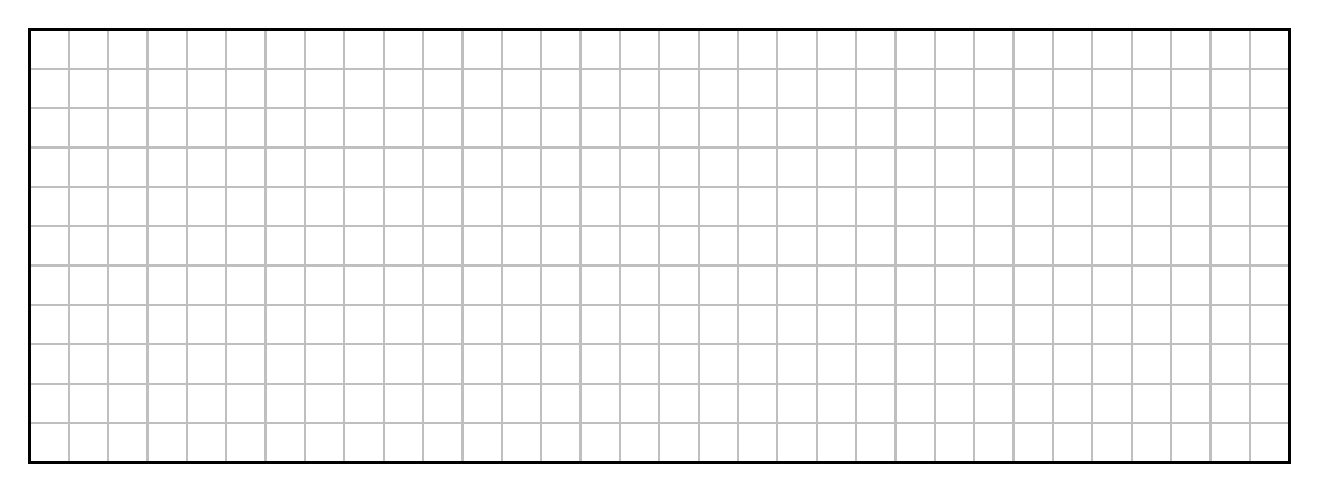
\begin{tikzpicture}
        % Define dimensions
        \def\gridwidth{32}
        \def\gridheight{11}
        \def\spacing{0.5}
        % Draw grid paper on the left
        \begin{scope}[xshift=0cm,yshift=0cm]
            % Major grid lines (thicker)
            \foreach \x in {0,1,...,\gridwidth}
                \draw[gray!50,thick] (\x*\spacing,0) -- (\x*\spacing,\gridheight*\spacing);
            \foreach \y in {0,1,...,\gridheight}
                \draw[gray!50, thick] (0,\y*\spacing) -- (\gridwidth*\spacing,\y*\spacing);
            \draw[black, very thick] (0,0) rectangle (\gridwidth*\spacing,\gridheight*\spacing);
        \end{scope}
    \end{tikzpicture}
\end{center}
What is the period of this wave?
Which direction is it moving?
How would you change $f(x,t)$ to make the wave move in the opposite direction?
\end{prelab}

% LAB SECTION
\begin{labsection}
\begin{objective}
    To measure the speed of sound in air, and to verify the dependence of string wave speed on the linear density of a string and the tension the string is under.
\end{objective}
\begin{theory}
    {\color{red} Hi this is terribel}
    Waves are ubiquitous in physics. They can be subdivided into two classes, \textsl{longitudinal} and \textsl{transverse} (see Fig.~\ref{fig: types of waves}). Acoustic waves (sound) are longitudinal waves, propagating via the collective motion of atoms within some \textsl{medium}, such as air. In such a longitudinal wave, the atoms oscillate parallel to the direction of motion of the wave. In contrast, in transverse waves, the medium oscillates perpendicular to the wave's direction of motion. Examples of transverse waves include a vibrating string that is fixed at both ends, surface waves on a body of water, and electromagnetic waves.

    \begin{figure}[ht]
        \centering
        
\includegraphics[width=0.8\linewidth]{Lab 11: The Speed of Waves/Wave Classification.png}
        \caption{Propagation of longitudinal waves (top) and transverse waves (bottom), showing the definition of wavelength $\lambda$ (center).}
        \label{fig: types of waves}
    \end{figure}

    Waves oscillate both in space and in time. Spatially, a wave is described by a wavelength $\lambda$, given in units of length, and an amplitude $A$, given in units that depend on the nature of the wave phenomenon. Temporally, the wave is described by its period $\tau$, which gives the time it takes for a wave to complete a single oscillation (or, if it's a traveling wave, to travel by a single wavelength). The inverse of the period is the wave's frequency $f$, given in units of Hertz (Hz) or seconds$^{-1}$, describing the number of cycles per second in the oscillation.
    
    The speed of a traveling wave $v$ satisfies
    %
    \begin{equation}\label{eq: wave speed}
        v = f\lambda.
    \end{equation}
    %
    While eq.~\ref{eq: wave speed} tells you how the frequency, wavelength, and wave speed are related, it does not explain why a given material supports a given wave speed.

    For example, longitudinal acoustic waves traveling through gases, fluids, and solids are affected by the compressibility of the medium, as defined by the bulk modulus\footnote{In solids, $K_s$ is called the coefficient of stiffness; in gases, it is called the modulus of bulk elasticity.} $K_s$, and the density of the medium, $\rho$. The speed of an acoustic wave will be
    %
    \begin{equation}\label{eq: acoustic wave speed}
        v = \sqrt{\frac{K_s}{\rho}}.
    \end{equation}
    %
    A 1D string of mass $M$ and length $L$, when pulled taught under tension $T$, will have a wave speed of
    %
    \begin{equation}\label{eq: string wave speed}
        v = \sqrt{\frac{T}{M/L}} = \sqrt{\frac{T}{\mu}},
    \end{equation}
    %
    where $\mu=M/L$ is the linear mass density. Stringed musical instruments support standing waves of fixed wavelength $\lambda$. Given the relationship between $f$, $\lambda$, and $v$ in eq.~\ref{eq: wave speed} and between $v$ and $T$ in eq.~\ref{eq: string wave speed}, you can see why musicians adjust the tension in their strings (``tuning'') until the desired frequencies emerge.

    \subsection*{Standing Waves}

    \begin{wrapfigure}[21]{r}{0.45\textwidth}
        \centering
        
\includegraphics[width=.9\linewidth]{Lab 11: The Speed of Waves/Harmonics.png}
        \caption{The first four harmonics of a standing wave.}
        \label{fig: standing wave harmonics}
    \end{wrapfigure}
    
    Several waves can occupy the same space at the same time and add together, leading to the phenomenon of \textbf{interference}. When the crests of two waves align, they add together, making a larger wave by \textsl{constructively} interfering with each other. When the peaks align with troughs, the waves cancel one another, \textsl{destructively} interfering.
    
    When two waves of the same amplitude and wavelength, but traveling in opposite directions, meet, they form a \textbf{standing wave}. This is what occurs when you pluck a string fixed at both ends. The plucking generates waves that move in opposite directions, hit the ends of the string,  reflect, and interfere with each other to produce a wave that looks like it isn't moving either to the left or to the right: a standing wave.
    
    When observing a standing wave on a string of length $L$, such as those shown in Figure~\ref{fig: standing wave harmonics}, one notices stationary points that do not move, such as where the ends are clamped. These stationary points are called \textbf{nodes}. Between every two nodes, there is a piece of string that moves with maximum amplitude, called an \textbf{antinode}.
    
    Because of the fixed \textsl{boundary conditions} on the string, only certain standing waves can be supported. The lowest-frequency standing wave, called the \textbf{fundamental frequency} or the first harmonic, corresponds to one half-wavelength ($L=\lambda/2$), with two nodes at the clamped ends and one antinode in the center. The next-highest frequency, called the second harmonic, corresponds to a full wavelength ($L=\lambda$) fitting on the string, with a node in the center. The third harmonic corresponds to $L=3\lambda/2$, with two nodes in the middle of the string between the fixed endpoints; the fourth harmonic corresponds to two wavelengths ($L=2\lambda$) with three nodes between the endpoints. And so on.

    It is also possible to set up standing longitudinal waves, for example, in air-filled tubes. Musical instruments such as organs, clarinets, flutes, and other tubes can be driven to resonance and support standing acoustic waves. At resonance, the tube will create a tone (the fundamental frequency) and overtones (the higher harmonics). If the tube is closed at one end, you will find an air displacement node (the air cannot oscillate against the boundary) and an air pressure antinode. At the open end of the tube is an air displacement antinode, since the air molecules at the opening oscillate longitudinally at maximum amplitude, and an air pressure node, since atmospheric pressure acts as a boundary condition at the opening.
    
    % When pushing someone on a swing, to make their amplitude grow you must push them at the correct moments.
    % The frequency of your pushing must be the same as the frequency of the swing to allow energy to be transferred.
    % This is the phenomenon of \textsl{resonance}.
    % In general everything vibrates.
    % If an object's harmonic matches the frequency of sound waves, then the little pushes caused by the longitudinal motion of the air molecules transfer kinetic energy into the object, increasing the amplitude of its vibration. 
    
\end{theory}

% \begin{equipment}
%     \item Sonometer
% \end{equipment}

\begin{experiment}
    \subsection*{Measuring Sound Speed in Air}
    
    In this experiment, you will measure the speed of sound indirectly by measuring the wavelength of a specific frequency of sound produced by a tuning fork. The resulting sound waves will enter a cylindrical cavity whose length you control, as shown in Figure~\ref{fig: tuning fork and cavity}. You will find the harmonics by changing the length of this cavity, which then allows you to infer the wavelength of the sound waves. With the frequency and wavelength measured, you can infer the sound speed using eq.~\ref{eq: wave speed}.

    \begin{figure}[ht]
        \centering
        
\includegraphics[width=0.85\linewidth]{Lab 11: The Speed of Waves/Experiment1_Overview.png}
        \caption{Tuning fork and open tube with an adjustable length $L$. The diagram shows the displacement waves of air.}
        \label{fig: tuning fork and cavity}
    \end{figure}

    \subsubsection*{Procedure}

    \begin{enumerate}
        \item Set up the apparatus as shown in Fig.~\ref{fig: tuning fork and cavity}. Position the tuning fork at the end of the plastic tube with its edge about \qty{1}{\centi\meter} from the open end of the tube.
        %
        \item Set up the piston close to the opening of the plastic tube to start the cavity length as small as possible.
        %
        \item Firmly strike the tuning fork with the rubber mallet. \textbf{Do not strike the fork on the table, or you could damage it.}
        %
        \item Move the piston away from the opening to increase the effective length of the resonant cavity. When you hear the tone suddenly get louder, you have reached a resonance and found an air displacement node.
        %
        \item Record the distance of each node from the open end of the tube in Data Table~\ref{data: sound speed} in the Postlab exercises. Include an estimate of the uncertainty of your measurements.
        %
        \item Record the frequency of the tuning fork in Data Table~\ref{data: sound speed}.
        %
        \item Repeat the previous steps with at least two other tuning forks with different frequencies.
    \end{enumerate}

    \subsection*{The Sonometer: Measuring Waves on a Stretched String}

    The sonometer is an apparatus used for exploring the wave properties of vibrating strings. It includes mounts to install strings of different linear densities $\mu$, a bridge that allows us to vary string length $L$, and weights that allow control of the tension $T$ in the strings. A schematic view of the sonometer is shown in Figure~\ref{fig: sonometer}.

    \begin{figure}[ht]
        \centering
        
\includegraphics[width=\linewidth]{Lab 11: The Speed of Waves/sonometer-schematic.png}
        \caption{The sonometer used to measure wave velocity on strings under tension. Image credit: PASCO Scientific.}
        \label{fig: sonometer}
    \end{figure}

    A \textbf{driver coil} connected to a function generator is used to generate standing waves on the string. The driver coil drives the string vibrations at any frequency the function generator will produce, but note that the frequency observed on the wire is usually \textbf{twice the driver frequency} because the driver electromagnet exerts a force on the wire twice per cycle. A \textbf{detector coil} allows you to view the vibration of the string on an oscilloscope.

    \begin{figure}[ht]
        \centering
        \setlength{\fboxsep}{0pt}
        \fbox{
\includegraphics[height=5.1cm]{Lab 11: The Speed of Waves/sonometer-adjust-screw.png}}
        \hfill
        \fbox{
\includegraphics[height=5.1cm]{Lab 11: The Speed of Waves/sonometer-tension-lever.png}}
        % 
\includegraphics[width=0.49\linewidth]{Lab 11: The Speed of Waves/sonometer-adjust-screw.png}
        % \hfill
        % 
\includegraphics[width=0.49\linewidth]{Lab 11: The Speed of Waves/sonometer-tension-lever.png}
        \caption{The sonometer adjustment screw (left) and tensioning lever (right). Credit: PASCO Scientific.}
        \label{fig: sonometer tension level}
    \end{figure}

    A set of color-coded strings with known and unknown linear mass densities is available in the lab. The strings and their properties are summarized in Table~\ref{tab: string properties}.

    \begin{table}[ht]
        \centering
        \renewcommand{\arraystretch}{1.2}
        \rowcolors{2}{gray!20}{white}
        \begin{tabular}{|c|>{\centering\arraybackslash}p{3.5cm}|>{\centering\arraybackslash}p{3.5cm}|}
            \hline
            \rowcolor{gray!20}
            \textbf{Color Code} & \textbf{Diameter} (inches) & \textbf{Linear Density} $\mu$ (\qty{}{\gram/\centi\meter})
            \\
            \hline
            White  & 0.010 & 0.39 \\ \hline
            Blue   & 0.014 & unknown \\ \hline
            Yellow & 0.017 & 1.12 \\ \hline
            Red    & 0.020 & unknown \\ \hline
            Black  & 0.022 & 1.84 \\ \hline
        \end{tabular}
        \caption{Properties of the strings used with the sonometer.}
        \label{tab: string properties}
    \end{table}

    \subsubsection*{Procedure: Measuring Wave Speed in a Wire of Known Density}

    \begin{enumerate}
        \item Set the amplitude of the function generator to its maximum value to see the largest string vibrations.

        \item Start with the bridges \qty{60}{\centi\meter} apart. Use any of the included strings with a known linear density (see Table~\ref{tab: string properties}) and hang a mass of approximately \qty{1}{\kilo\gram}, being sure to include the mass of the hanger itself, from the first slot of the tensioning lever (see Figure~\ref{fig: sonometer tension level}).
        
        \item Adjust the string adjustment knob so that the tensioning lever is horizontal. Position the driver coil \qty{5}{\centi\meter} from one of the bridges and position the detector coil near the center of the wire. Get the properties of the string you chose from Table~\ref{tab: string properties} and record the length, tension, and linear density of the string in Data Table~\ref{data: known wire}.

        \item Calculate the resonant frequency of the fundamental harmonic, $f_0$, using
        \[
            v = \lambda_0 f_0 = \sqrt{\frac{T}{\mu}}
        \]
        and record the result in Data Table~\ref{data: known wire}.

        \item Slowly increase the frequency of the signal to the driver coil, starting at \qty{25}{\hertz}. Listen for an increase in the volume of the sound from the sonometer and/or an increase in the size of the detector signal on the oscilloscope. Frequencies that result in the maximum string vibration are resonant frequencies. Determine the lowest frequency at which resonance occurs. This resonance is the first, or fundamental, harmonic. Estimate the frequency of the standing wave with the detector coil and oscilloscope by measuring the period, $\tau$, of the wave. The period is calculated by measuring the number of divisions between peaks in the oscilloscope display. There will be some uncertainty, $\Delta\tau$, from this measurement based on the precision with which you can read the period from the oscilloscope. The frequency $f=1/\tau$ is simply the inverse of the period. Record all results in Data Table~\ref{data: known wire}.

        \item Continue increasing the frequency of the driver coil to find successive resonant frequencies (at least 2 or 3). Think about how the frequencies and wavelengths for harmonics are related to the fundamental frequency and wavelength.

        \item Record the number of antinodes and the measured and calculated resonance frequency for each harmonic in Data Table~\ref{data: known wire}. Think about how the number of antinodes is related to the order of the harmonic.

        \item When done with the wire, put it back in the appropriate location.
    \end{enumerate}

    \subsubsection*{Procedure: Finding the Linear Density of an Unknown Wire}

    In this section of the lab, you will determine the linear density of an unknown wire using the sonometer.

    \begin{enumerate}
        \item Replace the wire on the sonometer with a color-coded unknown wire. Then, with the setup the same as in the previous section, measure the fundamental harmonic $f_0$ using 5 different tensions. Vary the tension by keeping the mass the same, but changing the location of the mass on the tensioning lever (use Figure~\ref{fig: sonometer tension level} as a reference). Change the string adjustment knob each time you move the mass so that the tensioning lever is always horizontal.

        \item Record the color code of the unknown wire, as well as the node spacing and the period of the wave as picked up by the detector coil using the oscilloscope, for each of the five tensions in Data Table~\ref{data: unknown wire}.

        \item When done with the wire, put it back in the appropriate location.

        \item Calculate the wave speed in Data Table~\ref{data: unknown wire velocity} and use it to compute the unknown linear mass density $\mu$ of the wire in the Postlab exercises.
    \end{enumerate}

\end{experiment}
\end{labsection}

\begin{postlab}

    \fullwidth{\subsection*{Measuring Sound Speed in Air (\pointsinrange{soundspeed} points)}}

    \begingradingrange{soundspeed}

    \filbreak
    \question[1] Record the frequency of the tuning forks and the distances to the first, second, and third nodes in Data Table~\ref{data: sound speed}.

    \begin{center}
        \captionsetup{font=normalsize}
        \captionof{data table}{Node lengths in the resonant air column, driven by a tuning fork. \label{data: sound speed}}
        \renewcommand{\arraystretch}{2}
        \begin{tabular}{|>{\centering\arraybackslash}p{2.25cm}|>{\centering\arraybackslash}p{2.75cm}|>{\centering\arraybackslash}p{2.75cm}|>{\centering\arraybackslash}p{2.75cm}|}
            \hline
            \rowcolor{gray!20}
            \textbf{Frequency} $f$ (Hz) & \textbf{Node Distance} $L_1$ (m) & \textbf{Node Distance} $L_2$ (m) & \textbf{Node Distance} $L_3$ (m)
            \\
            \hline
            & & & \\ \hline
            & & & \\ \hline
            & & & \\ \hline
        \end{tabular}
    \end{center}

    \filbreak
    \question[2] Calculate the average distance between consecutive nodes ($L_{i+1}-L_i$) for each frequency. This distance is $\lambda/2$ for the sound wave. Show a sample calculation below.
    %
    \begin{solution}[4cm]
    \end{solution}

    \endgradingrange{soundspeed}

    \filbreak
    \question[2] Calculate the speed of sound in air for each of the three tuning forks. Show your work.
    %
    \begin{solution}[4cm]
    \end{solution}

    \filbreak
    \question[2] From your three measurements of the sound speed, compute the average velocity of sound in air and its uncertainty using the standard deviation of your values. Show your work.
    %
    \begin{solution}[4cm]
    \end{solution}

    \endgradingrange{soundspeed}

    \filbreak
    \question[1] Using your value of the uncertainty from above, compare your results with the value resulting from the following formula for the speed of sound in dry air as a function of temperature:
    %
    \begin{align*}
        v(T) &\approx v_0\left(1 + 0.6T\right), & v_0 &= \qty{331.5}{\meter/\second} \text{ at \qty{0}{\celsius}},
    \end{align*}
    %
    where $T$ is the air temperature in degrees Celsius. (Note: room temperature is about \qty{20}{\celsius}).
    \begin{solution}[4cm]
    \end{solution}

    \endgradingrange{soundspeed}

\fullwidth{\subsection*{Sonometer: Standing Waves in a Wire of Known Density (\pointsinrange{known wire} points)}}

    \begingradingrange{known wire}

    \filbreak
    \question[1] Using eq.~\ref{eq: wave speed} and eq.~\ref{eq: string wave speed}, compute the resonant frequency of the fundamental harmonic. Show your work.
    %
    \begin{solution}[3cm]
    \end{solution}

    \filbreak
    \question[1] Record the number of antinodes and the resonant frequency (calculated and measured) for a given length of string $L$, a given tension $T$, and a given linear density $\mu$ in Data Table~\ref{data: known wire}.\\

    \begin{center}
        \begin{tabular}{r>{\raggedleft\arraybackslash}p{3cm}p{7mm}r>{\raggedleft\arraybackslash}p{3cm}p{7mm}r>{\raggedleft\arraybackslash}p{3cm}}
            $L=$ & m & & $T=$ & N & & $\mu=$ & kg/m
            \\
            \cline{2-2}\cline{5-5}\cline{8-8}
        \end{tabular}
    \end{center}

    \begin{center}
        \captionsetup{font=normalsize}
        \captionof{data table}{Measurements of the wire of known density. \label{data: known wire}}
        \renewcommand{\arraystretch}{2}
        \begin{tabular}{|>{\centering\arraybackslash}p{2.5cm}|>{\centering\arraybackslash}p{2.5cm}|>{\centering\arraybackslash}p{2.5cm}|>{\centering\arraybackslash}p{2.5cm}|>{\centering\arraybackslash}p{2.5cm}|}
        \hline
        \rowcolor{gray!20}
        Number of antinodes & Calculated resonant frequency (Hz) & Measured period $\tau$ (s) & Uncertainty in measured period $\Delta\tau$ (s) & Measured resonant frequency (Hz)
        \\
        \hline
        & & & & \\ \hline
        & & & & \\ \hline
        & & & & \\ \hline
        & & & & \\ \hline
        \end{tabular}
    \end{center}
    
    \endgradingrange{known wire}

\fullwidth{\subsection*{Sonometer: Standing Waves in a Wire of Unknown Density (\pointsinrange{unknown wire} points)}}

    \begingradingrange{unknown wire}

    \filbreak
    \question[1] Record the color code of the unknown wire below. In Data Table~\ref{data: unknown wire}, record the tension, the node spacing, and the period of the wave.

    \begin{center}
        \captionsetup{font=normalsize}
        \captionof{data table}{Measurements of the wire of unknown density. \label{data: unknown wire}}
        \renewcommand{\arraystretch}{2}
        \begin{tabular}{|>{\centering\arraybackslash}p{2.5cm}|>{\centering\arraybackslash}p{2.5cm}|>{\centering\arraybackslash}p{2.5cm}|>{\centering\arraybackslash}p{2.5cm}|}
        \hline
        \rowcolor{gray!20}
        Tension $T$ (N) & Node spacing (cm) & Period $\tau$ (s) & Uncertainty in period $\Delta\tau$ (s)
        \\
        \hline
        & & & \\ \hline
        & & & \\ \hline
        & & & \\ \hline
        & & & \\ \hline
        & & & \\ \hline
        \end{tabular}
    \end{center}

    \filbreak
    \question[3] Calculate the velocity and the uncertainty in the velocity of the wave for each of the five tensions using the measured wavelength and the period of the fundamental harmonic. (Hint: how do you relate the period of the fundamental harmonic as measured on the oscilloscope to its frequency?) Propagate the uncertainty in the period $\Delta\tau$ to the velocity using
    \[
        \Delta v=\frac{\Delta\tau}{\tau^2},
    \]
    which assumes the wavelength has no uncertainty. Compute the uncertainty in the square of the velocity as
    \[
        \Delta(v^2) = 2v\cdot\Delta v.
    \]
    Add your results to Data Table~\ref{data: unknown wire velocity}, showing work for one calculation out of the five.

    \begin{center}
        \captionsetup{font=normalsize}
        \captionof{data table}{Calculations of the wire of unknown density. \label{data: unknown wire velocity}}
        \renewcommand{\arraystretch}{2}
        \begin{tabular}{|>{\centering\arraybackslash}p{2.25cm}|>{\centering\arraybackslash}p{2.25cm}|>{\centering\arraybackslash}p{2.25cm}|>{\centering\arraybackslash}p{2.25cm}|>{\centering\arraybackslash}p{2.25cm}|>{\centering\arraybackslash}p{2.25cm}|}
        \hline
        \rowcolor{gray!20}
        Tension $T$ (N) & $\lambda$ (m) & $f$ (Hz) & $v$ (m/s) & $\Delta v$ (m/2) & $\Delta (v^2)$ (m$^2$/s$^2$)
        \\
        \hline
        & & & & & \\ \hline
        & & & & & \\ \hline
        & & & & & \\ \hline
        & & & & & \\ \hline
        & & & & & \\ \hline
        \end{tabular}
    \end{center}

    \begin{solution}[4cm]
        
    \end{solution}

    \filbreak
    \question[3] Plot $v^2$ versus $T$ in Graph~\ref{graph: unknown wire velocity}. Include labels, units, and the uncertainty on $v^2$ for each point.

    \begin{center}
    \captionsetup{font=normalsize}
    \captionof{graph}{Plot of $v^2$ vs. $T$. \label{graph: unknown wire velocity}}
    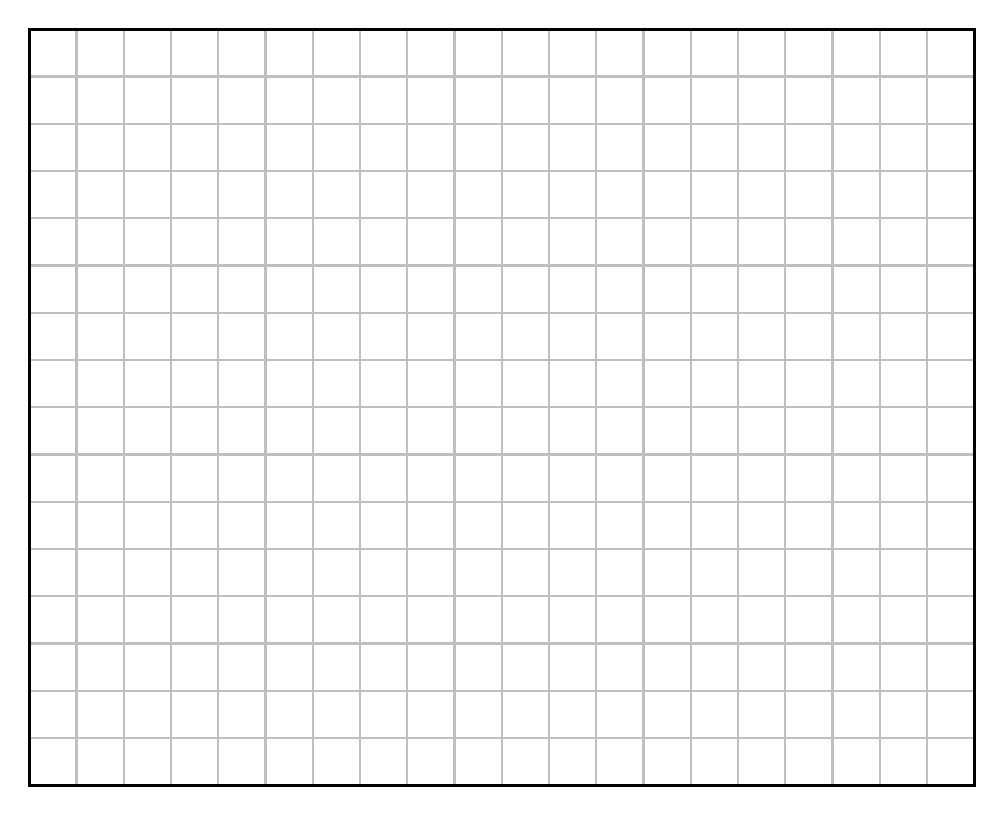
\begin{tikzpicture}
        % Define dimensions
        \def\gridwidth{20}
        \def\gridheight{16}
        \def\spacing{0.6}
        % Draw grid paper on the left
        \begin{scope}[xshift=0cm,yshift=0cm]
            % Major grid lines (thicker)
            \foreach \x in {0,1,...,\gridwidth}
                \draw[gray!50,thick] (\x*\spacing,0) -- (\x*\spacing,\gridheight*\spacing);
            \foreach \y in {0,1,...,\gridheight}
                \draw[gray!50, thick] (0,\y*\spacing) -- (\gridwidth*\spacing,\y*\spacing);
            \draw[black, very thick] (0,0) rectangle (\gridwidth*\spacing,\gridheight*\spacing);
        \end{scope}
    \end{tikzpicture}
    \end{center}

    \vspace{1cm}
    Is the relationship linear? Find the slope of the line. The slope is $1/\mu$, where $\mu$ is the linear density of the unknown wire. Show your work.
    %
    \begin{solution}[4cm]
        
    \end{solution}

    \filbreak
    \question[2] Calculate the uncertainty in $1/\mu$ as follows. In Graph~\ref{graph: unknown wire velocity}, draw the minimum and maximum slopes $m_\text{min}$ and $m_\text{max}$ that are consistent with the upper and lower error bars of the data. Use these slopes to compute an average slope and an uncertainty on the average:
    %
    \begin{align*}
        \overline{m} &= \frac{|m_\text{max} + m_\text{min}|}{2},
        \\
        \Delta\overline{m} &= \frac{|m_\text{max} + m_\text{min}|}{2}.
    \end{align*}
    %
    \begin{solution}[4cm]
        
    \end{solution}

    \filbreak
    \question[1] How does the value of $\mu$ from the slope compare to the accepted value of the color-coded wire? (Ask your TA for the accepted value of $\mu$ for your unknown wire.) Do the values agree within experimental uncertainties?
    %
    \begin{solution}[4cm]
        
    \end{solution}

    \endgradingrange{unknown wire}

%     \begin{center}
%     \begin{tikzpicture}
%     \begin{scope}[]
%     % Table headers
%     \node at (2, 0.3) [] {$f_1=$\hspace{3cm}};
%     \node at (5, 0.3) [] {$f_2=$\hspace{3cm}};
%     \node at (8, 0.3) [] {$f_3=$\hspace{3cm}};
%     \node at (11, 0.3) [] {$f_4=$\hspace{3cm}};
%     %\node at (5, 0.3) [] {$0.12$mm Plate};
%     %\node at (8, 0.3) [] {$0.60$mm Plate};
%     % Draw horizontal line under headers
%     \draw[thick] (-0.5, 0) -- (14, 0);
%      % Empty rows for data entry
%     \foreach \row in {1,...,3}
%     {
%         \node at (0.25, 0.3-0.6*\row) {$L_\row$};
%         \draw[color=gray] (-0.25, -0.6*\row) -- (13.75, -0.6*\row);
%     }
%     \draw[color=black] (-0.5, -0.6*3) -- (14, -0.6*3);
%     \node at (0.25, -1.5-0.6) {$\lambda$};
%     \node at (0.25, -1.5-0.6*2) {$c_S$};

%     \draw[color=gray] (-0.25, -1.75-0.6) -- (13.75, -1.75-0.6);
%     \draw[color=gray] (-0.25, -1.75-0.6*2) -- (13.75, -1.75-0.6*2);
%     \end{scope}  
% \end{tikzpicture} 
% \end{center}
% \subsection*{Question 1.1}
% Due to edge effects at the opening of the cavity, the first node in is not a goof measurement to use. However $L_2$ and $L_3$ are.
% How can you combine them to get the wavelength of the sound produced by each tuning fork?
% After writing that below, fill in the $\lambda$ row on the chart.
% \vspace{2cm}
% \subsection*{Question 1.2}
% Use the flambda equation to fill in the speed of sound, typically written $c_S$, row in the chart. 
% Use the four values to write down the measured speed of sound and the error of that measurement i.e. the unbiased estimators of the mean and standard deviation.
% \vspace{2cm}
% \subsection*{Question 1.3}
% In air, the speed of sound is dependent on temperature. 

\end{postlab}
\end{document}